\chapter{Examples of chapters}
\label{chap:examples}
\chaptoc{}
\newpage

% ~~~~~~~~~~~~~~~~~~~~
\section{The first section}
\label{sec:section1}

This is a thesis about the \gls{goto}.

I repeat, this is about \gls{goto}. There is currently only one \gls{goto}, but in the future there might be many more \gls{goto}s. \gls{goto} has a \gls{fov} of \about\SI{40}{\square\deg} and a mass of $\ll$ \SI{1}{\solarmass}.


\begin{figure}[htb]
\begin{center}
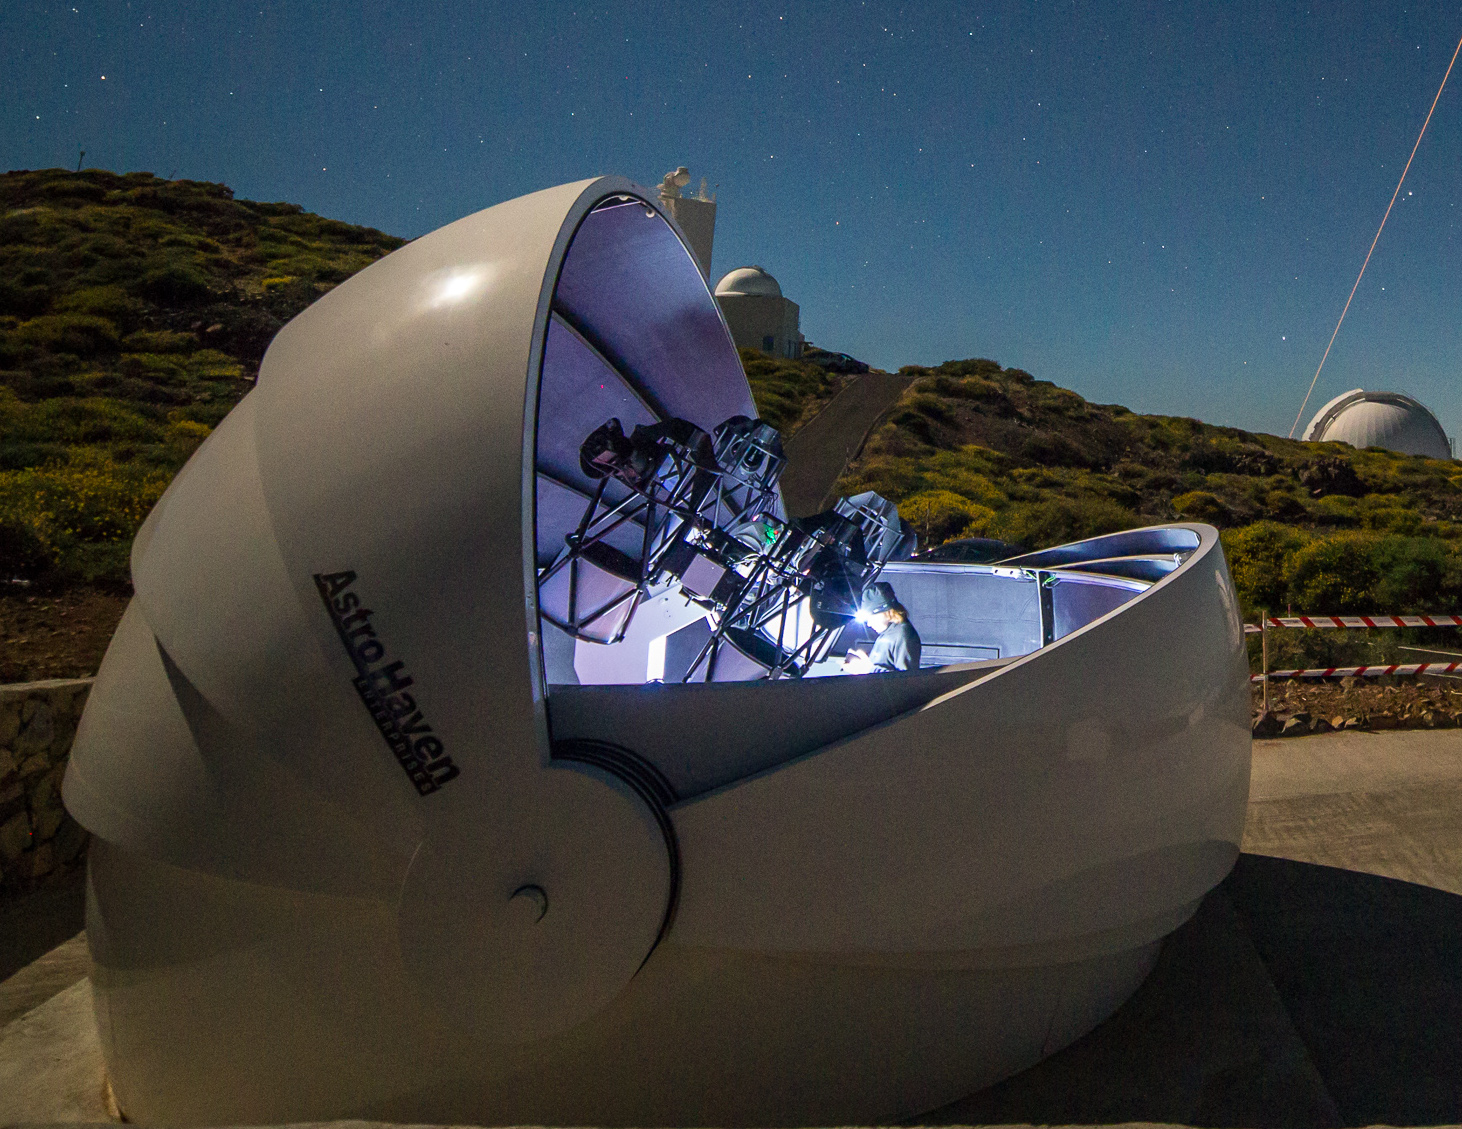
\includegraphics[width=11cm]{images/goto_photo.jpg}
\end{center}
\label{fig:goto_photo}
\caption[The GOTO prototype instrument]{The GOTO prototype instrument on La Palma, with four of the eventual eight unit telescopes.}
\end{figure}


\lipsum[1-2] % chktex 8

\subsection{A subsection}

\begin{table}[b]
\begin{center}
\begin{tabular}{c l}
~& \textbf{Target name} \\
\midrule
1 & GW181202 T4 \\
\end{tabular}
\end{center}
\label{tab:priority}
\caption[Some examples of calculated priority values]{Some examples of calculated priority values. In this example the weight factors are $a=1$, $p=10$, and $t=10$.}
\end{table}

\lipsum[3-6] % chktex 8

\subsection{And more}

\lipsum[7-9] % chktex 8

\subsubsection{No way, a subsub!}

\lipsum[10-12] % chktex 8


% ~~~~~~~~~~~~~~~~~~~~
\section{Another section}
\label{sec:section2}

\lipsum[13-19] % chktex 8
